\chapter{Kriptografski prilagodljiva komunikacija}
\label{ch:agility}

Pojam kriptografski prilagodljive komunikacije značajan je za sve sustave koji
aktivno koriste kriptografske protokole i temelj je svih današnjih
protokola za sigurnu komunikaciju. Kriptografski prilagodljiva komunikacija
predstavlja mogućnost promjene parametara s kojima se odvija komunikacija
bez mijenjanja sustava koji koristi kriptografiju za ostvarivanje sigurnosnih
zahtjeva.

Kriptografski prilagodljiva komunikacija mora podržavati mogućnost promjene
sljedeća dva parametra:
\begin{itemize}
    \item Kriptografskih algoritama s kojima se štiti
	komunikacija. Najčešće to uključuje više vrsta algoritama, npr.
	kriptografski sažetak i algoritam za digitalni potpis, ili skupove
	kriptografskih algoritama (engl. \emph{cryptographic suite}) poput
	protokola SSL~\cite{rfc6101} / TLS~\cite{rfc5246}.
    \item Ključeva koji će se koristiti s promijenjenim kriptografskim
	algoritmima. To se prije svega odnosi na tajne ključeve koji se koriste
	za simetrično šifriranje i izračunavanje MAC algoritama, dok se javni
	ključevi rjeđe mijenjaju. Različiti kriptografski algoritmi koriste
	ključeve različitih duljina i potrebno je za svaku novu komunikaciju
	promijeniti kriptografski ključ koji se koristi (engl. \emph{key
	separation} \cite{krawczyk1996skeme}).
\end{itemize}
Glavne prednosti kriptografski prilagodljive komunikacije su sljedeće:
\begin{itemize}
    \item Omogućuje korištenje različitih ostvarenja kriptografskih
	algoritama koje ne moraju biti sastavni dio postavljenog sustava.
    \item Mogućnost brze promjene kriptografskih algoritama koji imaju određene
	probleme u samom algoritmu ili korištenom programskom ostvarenju.
    \item Uvođenje novih i sigurnijih kriptografskih algoritama u sustav na
	jednostavan način koji ne utječe na trenutnu konfiguraciju sustava.
    \item Prilagođavanje sustava novim kriptografskim zahtjevima koje zahtjeva
	napredak metoda napada na kriptografske algoritme ili proces
	certifikacije sustava.
    \item Veća razina prilagodljivosti koja omogućuje komunikaciju s uređajima
	različitih računalnih sposobnosti koji podržavaju razne kriptografske
	algoritme. 
\end{itemize}

U nastavku ovog poglavlja dan je pregled postojećih protokola koji koriste
kriptografski prilagodljivu komunikaciju kako bi ostvarili potrebne sigurnosne
zahtjeve. Uz to, istaknute su njihove glavne prednosti i nedostaci.

\section{Pregled kriptografski prilagodljivih protokola}

Kriptografija je najviše zastupljena u području zaštite mrežne komunikacije
korištenjem protokola koji omogućavaju sigurne komunikacijske kanale (engl.
\emph{secure channel protocols}). Usporedba predloženog protokola ACAP (engl.
\emph{Agile Cryptographic Agreement Protocol}) i
standardiziranih protokola prikazana je u tablici \ref{tab:comparison}.
Početna ideja iza protokola ACAP na protokolu SEND \cite{rfc3971} (engl.
\emph{Secure Neighbor Discovery}) prikazana je u \cite{vasic2011deploying}.
Neovisnost o sloju i daljnja razrada principa dogovora opisana je u radu
\cite{ACNP}. Posljednje proširenje protokola koje uključuje formate svih poruka
i formalno verificirani model prezentirano je u radu
\cite{vasic2016lightweight}.

Prvi stupac sadrži imena protokola, a drugi stupac sadrži
podatak o parametrima koji se dogovaraju u protokolu. Dogovor
kriptografskih algoritama i ključeva bi se u pravilu trebao ostvariti u sklopu
istog dogovora jer se ključevi ne mogu koristiti bez dogovorenih algoritama.
Samo protokol JFK~\cite{aiello2004jfk} (engl. \emph{Just Fast Keying}) služi za
dogovor ključeva jer se dogovor
algoritama odvija u sklopu protokola IPsec~\cite{rfc4301} koji ga koristi. U
trećem stupcu nalaze se podaci o sloju na kojem se protokoli mogu koristiti.
Protokol ACAP, koji je opisan u doktorskoj disertaciji, jedini je protokol
koji se može koristiti neovisno o komunikacijskom sloju.

\begin{table*}[hbt]
\caption{Pregled kriptografski prilagodljivih protokola}
\renewcommand{\arraystretch}{1.3}
\label{tab:comparison}
\centering
\small
\begin{tabular}{p{2.2cm} p{1.9cm} p{2.3cm} p{3.7cm} p{1.4cm} p{1.9cm}}
\hline
Ime\newline protokola &
    Dogovoreni parametri &
    Komunikacijski sloj &
    Namjena &
    Složenost &
    Formalna verifikacija
    \\ \hline \hline
ACAP
    & ključ i\newline algoritmi
    & svi slojevi
    & dogovor ključa\newline i algoritama
    & niska
    & da
    \\ \hline
JFK\textsuperscript{\cite{aiello2004jfk}}
    & ključ
    & vezan uz IPsec
    & dogovor ključeva
    & niska
    & da
    \\ \hline
IPsec\textsuperscript{\cite{rfc4301}}
    & ključ i\newline algoritmi
    & sloj IP
    & zaštita prometa, VPN
    & visoka
    & djelomična
    \\ \hline
SSL\textsuperscript{\cite{rfc6101}}/TLS\textsuperscript{\cite{rfc5246}}
DTLS\textsuperscript{\cite{rfc6347}}
    & ključ i\newline algoritmi
    & transportni sloj (TCP, UDP)
    & sigurni komunikacijski kanali
    & visoka
    & djelomična
    \\ \hline
MinimaLT\textsuperscript{\cite{petullo2013minimalt}}
    & ključ i\newline algoritmi
    & UDP
    & sigurni komunikacijski kanali
    & srednja
    & djelomična
    \\ \hline
SSH\textsuperscript{\cite{rfc4251}}
    & ključ i\newline algoritmi
    & aplikacijski sloj
    & sigurni komunikacijski kanali i ljuska (\emph{shell})
    & srednja
    & djelomična
    \\ \hline
Tcpcrypt\textsuperscript{\cite{bittau2010tcpcrypt}}
    & ključ i\newline algoritmi
    & TCP
    & sigurni komunikacijski kanali putem TCP-a
    & srednja
    & ne
    \\ \hline
QUIC\textsuperscript{\cite{roskind2013quick}}
    & ključ i\newline algoritmi
    & UDP
    & siguran prijenos HTTP prometa
    & srednja
    & ne
    \\ \hline
\end{tabular}
\end{table*}

Četvrti stupac
opisuje namjenu protokola, a peti stupac sadrži opis složenosti protokola.
Složenost protokola izravno je ovisna o njegovoj namjeni. Namjena utječe na broj
komponenti protokola, a broj komponenti određuje složenost protokola. Na
primjer,
SSL~\cite{rfc6101} / TLS~\cite{rfc5246} sastoji se od 4 komponente, a IPsec i
SSH~\cite{rfc4251} od 3 komponente. S druge strane QUIC~\cite{roskind2013quick},
Tcpcrypt~\cite{bittau2010tcpcrypt} i MinimaLT~\cite{petullo2013minimalt}
sastoje se od dvije komponente, jedna za razmjenu ključeva i druga za siguran
prijenos podataka. Složenost protokola ključan je aspekt protokola jer otežava
programsko ostvarenje protokola i izglede za uspješnim formalnim modeliranjem i
verifikacijom. Dostupnost provedene formalne verifikacije navedena je u
posljednjem stupcu.

\subsection{Protokoli SSL/(D)TLS}
Protokoli SSL~\cite{rfc6101} i TLS~\cite{rfc5246} omogućavaju sigurnu komunikaciju
putem pouzdane veze koja koristi protokol TCP (engl. \emph{Transmission Control
Protocol}) za prijenos podataka. Osim protokola i komunikacijske logike u
SSL/TLS rješenjima nalaze se i svi kriptografski algoritmi koji će se
koristiti za zaštitu prenesenih podataka. To otežava promjenu programskog
ostvarenja algoritma u sustavu.
Oba protokola dizajnirana su na kraju prošlog stoljeća i njihovi su temelji
postavljeni u vrijeme kada je znanje o dizajnu sigurnih protokola i kriptografskih
algoritama
bilo značajno manje od trenutka pisanja disertacije.
SSL/TLS arhitektura je složena i sastoji se od više protokola:
\begin{itemize}
    \item Protokol za dogovor početnih parametara komunikacije (engl.
	\emph{Handshake protocol}),
    \item Protokol za promjenu parametara komunikacije (engl. \emph{Change
	Cipher Spec protocol}),
    \item Protokol za upravljanje podacima (engl. \emph{Record protocol}) i
    \item Protokol za dojavu grešaka u komunikaciji (engl. \emph{Alert
	protocol}).
\end{itemize}
Cjelokupna arhitektura SSL/TLS protokola prikazana je na slici
\ref{fig:tls_proto}.

\begin{figure}[hbt]
    \centering
\begin{bytefield}[bitwidth=1em, bitheight=4em]{32}
    \bitbox{8}{\emph{Handshake} protokol} & \bitbox{8}{\emph{Change Cipher Spec} protokol} &
    \bitbox{8}{\emph{Alert} protokol} & \bitbox{8}{Protokoli viših slojeva (HTTP, ...)} \\
    \wordbox{1}{\emph{Record} protokol} \\
    \wordbox{1}{TCP}
\end{bytefield}
\caption{Arhitektura protokola SSL/TLS}
\label{fig:tls_proto}
\end{figure}

Zbog složenosti arhitekture protokola i velikog broja komponenti potrebnih
za ostvarivanje sigurne komunikacije počeli su se pronalaziti problemi u dizajnu
protokola kao i u programskim ostvarenjima protokola SSL/TLS. U \cite{duong2011here}
prikazana je ranjivost CBC načina šifriranja dok \cite{be2013crime} opisuje
problem koji se javlja zbog krivog načina korištenja kompresije prilikom
šifriranja. Uz to otkrivene su ranjivosti u protokolu za upravljanje podacima
\cite{paterson2013luck13} i korištenja šifre RC4 za generiranje nasumičnih
vrijednosti~\cite{paterson2013rc4}. Dodatno su se počele javljati i
ranjivosti programskih ostvarenja koje su omogućile napad Heartbleed (OpenSSL)
\cite{durumeric2014matter} i razne
druge napade na sustav za upravljanje certifikatima (Apple)
\cite{bland2014finding}.

Iako protokol SSL/TLS predstavlja temelj moderne sigurne komunikacije putem
Interneta jedan od osnovnih problema leži u kompleksnosti protokola i njegovog
dizajna. Problem bi bio puno manje izražen kada bi kriptografski algoritmi bili
odvojeni od sustava komunikacije i kada bi dizajn protokola bio pojednostavljen
na način da podržava samo sigurne načine dogovora i zaštite komunikacije, koje ne
bi
uključivale trenutno nesigurne algoritme i načine dogovora (SSLv2, SSLv3).

Protokol DTLS~\cite{rfc6347} predstavlja prilagodbu protokola TLS za datagramsku
komunikaciju putem protokola UDP i DCCP\@. On dodaje razne mehanizme za
prilagodbu sigurne komunikacije datagramskom načinu komuniciranja koji uključuje
retransmisiju poruka tijekom dogovaranja parametara komunikacije i brine se za
održavanje redoslijeda poruka tijekom komunikacije.

\subsection{Protokol IPsec}
IPsec~\cite{rfc4301} predstavlja skup kriptografskih mehanizama koji služi za
uspostavljanje sigurne komunikacije kroz
nesigurnu mrežu. Najčešće se koristi za povezivanje udaljenih računala na
siguran način do odredišne mreže preko Interneta. Sastoji se od više različitih
protokola i skupa kriptografskih algoritama. 

Protokol IPsec se može podijeliti u tri osnovne kategorije:
\begin{itemize}
    \item protokoli za zaštitu mrežnog prometa, AH (engl. \emph{Authentication
	Header})
	i ESP (engl. \emph{Encapsulating security Payload}),
    \item sustav za upravljanje ključevima i parametrima za sigurnu
	komunikaciju što uključuje upravljanje sigurnosnim asocijacijama (engl.
	\emph{Security Association}, SA) i
    \item sustav za određivanje koji promet treba biti zaštićen i s kojim
	parametrima što je izravno definirano s trenutno uspostavljenim SA u
	sustavu.
\end{itemize}

U standardu IPsec važan je pojam skupa kriptografskih algoritama
(engl. \emph{cryptographic suite}) koji predstavlja više različitih vrsta
algoritama, poput algoritama za šifriranje, osiguravanje integriteta,
Diffie-Hellman parametara i različitih funkcija za generiranje pseudo nasumičnih
brojeva (npr. AES za šifriranje, SHA-256 za integritet, ...).

Protokol AH uključen je u IPsec standard iz povijesnih razloga, dok se protokol
ESP koristi za šifriranje i autentifikaciju prometa koji se razmjenjuje.
Zaštita se može provoditi na dva načina: transportni i tunelirani. Transportni
način štiti samo sadržaj paketa bez promjene zaglavlja. Taj se način prijenosa
koristi za zaštitu komunikacije između dvije krajnje točke u mreži. Tunelirani
način rada štiti cijelo originalno zaglavlje tako da cijeli
paket enkapsulira pod novim zaglavljem dok se na odredištu sadržaj paketa
dekapsulira i šalje u istom početnom obliku. Ovaj se način prijenosa uspostavlja
u dva scenarija:
\begin{itemize}
    \item između dva čvora koji nisu krajnje točke u komunikaciji i omogućuje
    zaštićeno prosljeđivanje svog prometa iz jednog mrežnog segmenta u drugi;
    VPN između dva mrežna segmenta i
\item između jednog čvora koji je krajnja točka u komunikaciji i želi
    komunicirati s mrežnim segmentom koji se nalazi u zaštićenoj mreži; VPN
    veza udaljenog klijenta u zaštićeni mrežni segment.
\end{itemize}
Cjelokupna zaštita prometa provodi se na temelju dogovorenih sigurnosnih
asocijacija, a proces zaštite prometa odvija se u jezgri operacijskog sustava
računala koji provodi zaštitu.

Protokol IKE~\cite{rfc5996} (engl. \emph{Internet Key Exchange}) služi za
dogovor parametara za sigurnu komunikaciju i
upravlja trenutno aktivnim sigurnosnim asocijacijama (SA). To je samostalan
protokol koji omogućuje
kriptografski prilagodljivu komunikaciju i dinamičko dogovaranje kriptografskih
parametara za zaštitu komunikacije. Bez protokola IKE ne bi bio ostvariv
automatski dogovor sigurnosnih asocijacija te bi se sve SA trebale ručno
podešavati. Stoga protokol IKE izravno omogućuje široku primjenu i korištenje
cjelokupnog standarda IPsec za zaštitu prometa koji se prenosi
između dvije podmreže koje su povezane putem Interneta.

Posljednji dio IPsec-a nalazi se u jezgri operacijskog sustava koji se bavi
odlučivanjem o tome koji se podaci štite, ovisno o adresama i
protokolima koji se koriste za komunikaciju. U jezgri operacijskog sustava uz
to se nalaze i kriptografski mehanizmi s pomoću kojih se štiti promet.

Cjelokupni standard IPsec omogućuje ostvarivanje sigurnosnih zahtjeva tajnosti i
integriteta cjelokupnog prometa koji se prenosi s pomoću protokola IP. Samim
time, to je složen sustav koji se sastoji od većeg broja komponenti koje se
protežu od jezgre operacijskog sustava, kako bi se omogućilo rukovanje
prometom, do korisničkih aplikacija koje omogućavaju automatizirano podešavanje
sigurne komunikacije.

IPsec je složen sustav koji ima važne primjene, ali razina sigurnosti koju pruža
nije uvijek potrebna i nije uvijek izvediva uz zadovoljavajuću razinu
performansi. Uz to IPsec je čvrsto vezan uz operacijski sustav i promjene u
slučaju sigurnosnih problema zahtijevaju potencijalno velike zahvate na
cjelokupnom sustavu. Zaštita mrežnog prometa IPsec-om moguća je između računala i
mobilnih uređaja nove generacije, ali je teško primjenjiva na uređajima u
okolini Interneta stvari koji imaju značajno manje računalne mogućnosti.

\subsubsection{Protokol JFK}
\label{sec:jfk}

Protokol JFK (engl. \emph{Just Fast Keying})~\cite{aiello2004jfk} bio je
predložen kao alternativa protokolu IKE verzije 1 i postao je standardni dio
trenutne verzije protokola IKE, IKE verzije 2. Razlog tomu su ranjivosti koje su
otkrivene u protokolu IKE verzije 1 \cite{canetti2002verif}. U protokolu JFK koristi se
SIGMA princip za zaštitu dogovora i razmjene ključeva te služi prije svega za
dogovor oko sigurnosnih asocijacija. Uz to dodatno omogućuje zaštitu identiteta
jedne od komunicirajućih strana. Zaštita identiteta je važan parametar u
komunikaciji, ali se rijetko javlja potreba za tim zahtjevom.

\no{
IKE (Internet Key Exchange)~\cite{rfc5996} is a standalone protocol
that is part of the IPsec protocol suite. It is used for exchanging keys and
agreeing upon Security Associations for securing network communication. It is a
well known and tested protocol but it is not lightweight and provides more
mechanisms that can be done separately from key exchange and cryptographic
algorithm agreement~\cite{aiello2004jfk}.


JFK (Just Fast Keying)~\cite{aiello2004jfk} proposes an
alternative to IKE~\cite{rfc5996} key exchange protocol that ensures identity
protection for either the responder or the receiver.
The main differences with ACAP are as follows.
We allow for negotiation of cryptographic algorithms.
Our communicating parties are equal peers and can be used
for all layers and applications. Since identity protection is not included our
messages are somewhat simpler and take a different approach while using the same
sign-and-mac principles. For our purposes we need two round trip times to establish
cryptographic keys and
algorithms.
}

\subsection{Protokol SSH}
\label{sec:ssh}
Protokol SSH~\cite{rfc4251} je standardni protokol za upravljanjem udaljenim
računalima korištenjem komandno-linijskog sučelja za izvođenje naredbi, prenošenje
datoteka i sigurno tuneliranje mrežnog prometa između dva računala.

Protokol SSH sastoji se od 3 protokola:
\begin{itemize}
    \item Protokol za upravljanje prijenosom podataka (engl. \emph{SSH
    Transport Layer protocol}) koji se brine za osiguravanje
    cjelovitosti i tajnosti podataka pri prijenosu kroz mrežu \cite{rfc4253}.
    \item Protokol za upravljanje vezama (engl. \emph{SSH Connection protocol})
    koji je zadužen za multipleksiranje više tokova podataka kroz istu SSH vezu
    (npr. istodobno udaljeno upravljanje uz prijenos podataka) \cite{rfc4254}.
    \item Protokol za autentifikaciju korisnika (engl. \emph{SSH User
    Authentication protocol}) koji provjerava korisnikove podatke i određuje
    ima li korisnik pravo pristupa sustavu (računalu) \cite{rfc4252}.
\end{itemize}

Protokol SSH se izvodi kroz TCP vezu između dva računala u mreži, a međusobni
odnosi sastavnih dijelova protokola SSH prikazani su na slici
\ref{fig:ssh_proto}.

\begin{figure}[hbt]
    \centering
\begin{bytefield}[bitwidth=1em, bitheight=2em]{32}
    \bitbox{16}{SSH \emph{User Authentication} protokol} & \bitbox{16}{SSH \emph{Connection} protokol} \\
    \wordbox{1}{SSH \emph{Transport Layer} protokol} \\
    \wordbox{1}{TCP}
\end{bytefield}
\caption{Arhitektura protokola SSH}
\label{fig:ssh_proto}
\end{figure}

Protokol SSH u sklopu upravljanja prijenosom podataka dogovara kriptografske
ključeve i algoritme koji će se koristiti za zaštitu komunikacije. Odluka o
kriptografskim algoritmima izvodi se na sljedeći način:
\begin{itemize}
\item Klijent i poslužitelj razmijene uređene liste podržanih algoritama.
\item Odabire se prvi algoritam koji se nalazi na popisu klijenta, a ujedno je
podržan od strane poslužitelja.
\item U slučaju da se ne može pronaći zajednički algoritam veza se prekida.
\end{itemize}
Protokol SSH dogovara način razmjene ključeva, asimetrični algoritam šifriranja,
simetrični algoritam šifriranja, algoritam za autentifikaciju poruka (engl.
\emph{message authentication algorithm}) i algoritam kriptografskog sažetka. 

\subsection{Protokoli nove generacije}
Protokol tcpcrypt~\cite{bittau2010tcpcrypt} predstavlja novi pristup zaštiti
prometa koji se razmjenjuje putem protokola TCP. Nastao je kao moguće rješenje
na probleme koji se pojavljuju prilikom korištenja protokola SSL/TLS\@.
Postupak dogovaranja parametara za sigurnu komunikaciju integriran je u
standardnu sinkronizaciju u tri koraka (engl. \emph{three-way handshake}) s
dodatkom jedne dodatne poruke. Uspostava sigurne veze može se uspostaviti u 2
vremena povrata (engl. \emph{Round Trip Time} - RTT) dok je kod TLS-a potrebno
barem 3 RTT-a. Opterećenje poslužitelja se isto značajno smanjuje jer se
postupak asimetričnog šifriranja premješta na klijenta. Stoga, tcpcrypt
je efikasnije rješenje, u odnosu na TLS, za zaštitu prometa koji se
izmjenjuje protokolom TCP. Smanjena kompleksnost protokola omogućava lakše
održavanje i razvijanje protokola te smanjuje mogućnosti grešaka u dizajnu i
programskom ostvarenju.

Protokol QUIC~\cite{roskind2013quick} je novi pristup sigurnom prijenosu
podataka putem protokola HTTP korištenjem protokola UDP kao transportnog
protokola. UDP se koristi kako bi se smanjila kašnjenja i opterećenja na
poslužiteljima. Trenutno je integriran u preglednik sjedišta weba Chromium kako
bi se
omogućio lakši razvoj i testiranje. QUIC uvodi nove mehanizme zaštite od
lažiranja adresa IP i napada ponavljanjem prometa.

\comment{ QUIC adapts the same
method of lowering server load by using the same DH exponential for a period of
time and precomputing certain message parts. A similar approach is taken in JFK 
and ACAP.
}

Protokol MinimaLT~\cite{petullo2013minimalt} je jedan od protokola nove
generacije sličan QUICu, koji je dizajniran da pruža veću razinu sigurnosti
tako da se Diffie-Hellman parametri i javni ključevi dijele s pomoću DNS upita
i odgovora \cite{freire2013non}. Komunicirajuće strane međusobno se
autentificiraju korištenjem javnih ključeva. MinimaLT postiže veću razinu
fleksibilnosti zbog prijenosa podataka protokolom UDP umjesto protokolom TCP,
ali je i dalje primjenjiv isključivo na slojevima iznad transportnog.

\comment{ A new
non-interactive key exchange approach \cite{freire2013non} is used to minimize RTTs while
establishing secure connections. MinimaLT gains more flexibilty by transferring
all data by UDP instead of TCP but is strictly tied to the transportation layer. 
}

\section{Dogovor zajedničke tajne i kriptografskih algoritama}

Dogovor zajedničke tajne u postojećim se protokolima izvodi korištenjem
asimetričnih algoritama. Dogovor se može izvoditi korištenjem protokola
Diffie-Hellman ili korištenjem asimetričnih algoritama (npr. RSA) za postizanje
tajnosti korištenjem principa digitalne omotnice. U oba slučaju razmjenuju se
dijelovi s kojima se izračunava zajednička tajna. Kod korištenja Diffie-Hellman
algoritma dijelovi koji se razmjenjuju su javni, a kod korištenja digitalne
omotnice dijelovi su tajni.

Protokoli SSL/TLS podržavaju oba načina razmjene ključeva, dok SSH, IPsec, QUIC i
MinimaLT koriste Diffie-Hellman za uspostavu početne tajne, a  tcpcrypt koristi
samo princip digitalne omotnice. IPsec razmjena koristi princip SIGMA u 
protokolu JFK koji je sličan principima korištenima u protokolu ACAP.
Odluka o kriptografskim algoritmima se kod protokola SSL/TLS, SSH, tcpcrypt i
QUIC odrađuje na način da komunicirajuće strane razmijene podržane algoritme
koji su raspoređeni uzlazno po njihovim jačinama. U pravilu se uzima prvi
algoritam na popisu klijenta koji je podržan od strane poslužitelja.

\subsection{Novi algoritmi dogovora zajedničke tajne}

Uz princip SIGMA za autentificirano dogovaranje zajedničke tajne, postoje noviji
algoritmi koji koriste implicitnu autentifikaciju bez potrebe izračuna i
provjere digitalnih potpisa. Tim algoritmima potrebno je dvije poruke za dogovor
zajedničke tajne umjesto tri poruke, ali je njihov dizajn puno
osjetljiviji u odnosu na eksplicitno autentificirane protokole
\cite{yao2013oake}. To su algoritmi zasnovani na principu MQV
(Menezes–Qu–Vanstone)\cite{law2003efficient} i OAKE (engl. \emph{Optimal
(implicitly) Authenticated (Diffie-Hellman) Key-Exchange}) \cite{yao2013oake}.

Početni MQV princip proširen je u vidu HMQV (engl. \emph{Hashed MQV})
\cite{krawczyk2005hmqv} zbog početnih napada na taj princip. Dodatnim
istraživanjem pronađene su nove ranjivosti na napad čovjek u sredini koje su
riješene uvođenjem principa FHMQV (engl. \emph{Fully Hashed MQV})
\cite{sarr2010secure}. FHMQV predstavlja formalno verificirani princip koji
omogućuje siguran dogovor zajedničke tajne \cite{liu2014security}. FHMQV se u
vrijeme pisanja doktorske disertacije počeo aktivno koristiti u sklopu drugih
rješenja i protokola \cite{gruber2014concept} \cite{barenghi2014snake}. Dodatno
se aktivno istražuju novi MQV principi koji se temelje na eliptičnim krivuljama
(ECMQV) ili su posebno prilagođeni uređajima s ograničenim mogućnostima
\cite{zhao2015shmqv}.
Kao alternativa MQV principu izveden je OAKE princip koji pruža određene
prednosti u vidu smanjivanja zahtjevnosti izračuna zajedničke tajne i zaštite
identiteta komunicirajućih strana \cite{yao2013oake}. Primjena OAKE principa je
nedavno prepoznata u sklopu određenih protokola i primjena
\cite{dagdelen2013cryptographic}.

Osnovna prepreka u korištenju novih algoritama za autentificirani dogovor
zajedničke tajne je nepostojanje standardnog programskog rješenja navedenih
principa u
sklopu kriptografskih biblioteka, što onemogućava praktično ostvarenje i
mjerenje utjecaja kriptografskih izračuna u odnosu na mrežnu komunikaciju. Drugi
nedostatak povezan je s izostankom javnih ključeva (certifikata) u
razmjeni što onemogućuje provjeru identiteta u sustavima koji se oslanjaju na
infrastrukturu javnog ključa (engl. \emph{Public Key Infrastructure} - PKI).
Kroz buduće istraživanje napretka implicitno autentificiranih Diffie-Hellman
protokola za dogovor zajedničke tajne (engl. \emph{Implicitly Authenticated
Diffie Hellman Key Exchange} - IADHKE) te pažljivi dizajn i verifikaciju novog
rješenja mogao bi se unaprijediti mehanizam za dogovor zajedničke tajne u
protokolu ACAP na način koji bi zahtijevao manje resursa i potencijalno manji
broj poruka za dogovor svih parametara.

\nomenclature{PKI}{\emph{Public Key Infrastructure} - infrastruktura javnog
ključa}

\section{Kriptografska prilagodljivost u okolini Interneta stvari}

Svi trenutno programski ostvareni protokoli koji su navedeni u tablici
\ref{tab:comparison} imaju kompleksnu arhitekturu koja omogućuje sigurnu
komunikaciju korištenjem komunikacijskih kanala. Uspostava sigurnih
komunikacijskih kanala i njihovo održavanje zahtijeva dodatne resurse, a često
nisu potrebni u okolini Interneta stvari. Komunikacija u okolini Interneta
stvari u pravilu je temeljena na porukama koje nose određenu informaciju
(npr. izmjereni podatak iz okoliša, naredbu za upravljanje uređajima ili
podatke za ažuriranje uređaja).

Arhitektura Interneta stvari je slojevita i sastoji se od mnoštva različitih
uređaja koji se mogu rasporediti u različite skupine ovisno o njihovim trenutnim
mogućnostima, poput računalnih sposobnosti, pristupa napajanju i propusnosti
mrežne komunikacije. Na slici \ref{fig:iot1} prikazana je arhitektura Interneta
stvari \cite{perera2014context} i tri
osnovna sloja arhitekture. Senzori predstavljaju najviše ograničenu
skupinu uređaja, srednji sloj predstavlja djelomično ograničenu skupinu, dok
sloj računalnog oblaka ima neograničen pristup resursima. Zbog velikog raspona
različitih mogućnosti uređaja u okolini Interneta stvari nužno je ostvariti
prilagodljivi algoritam koji će uzimati u obzir trenutne mogućnosti uređaja za
odabir kriptografskih algoritama. Trenutni algoritmi dogovora algoritama uzimaju
u obzir samo razinu sigurnosti što može negativno utjecati na brzinu
komunikacije i potrošnje izvora napajanja.

\begin{figure}[htb]
    \centering
    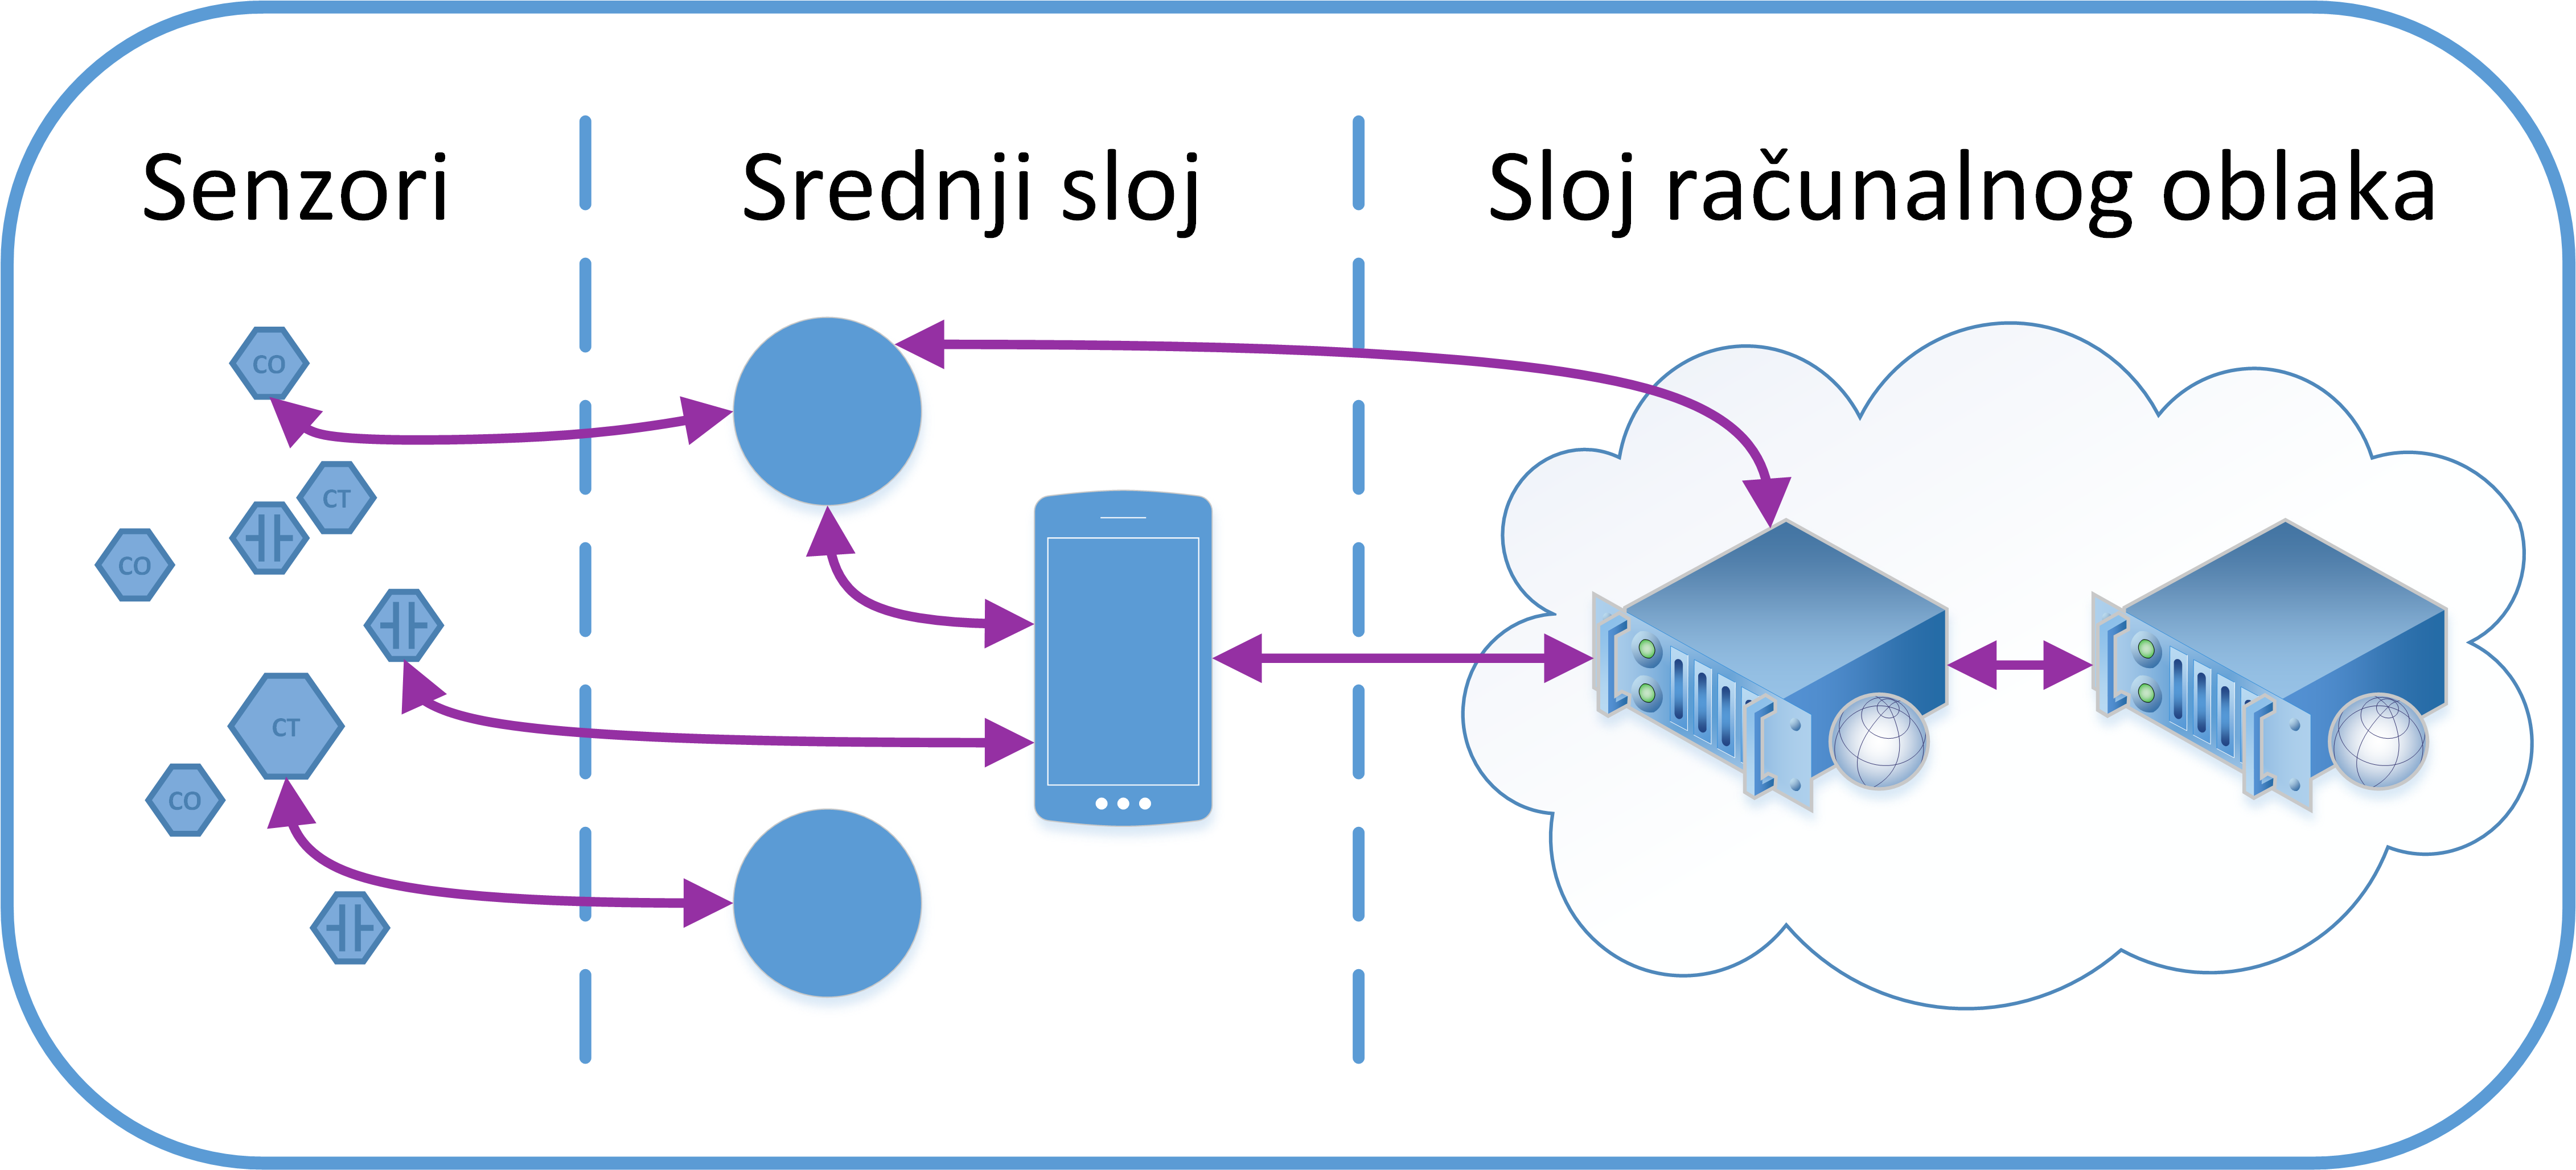
\includegraphics[width=0.6\textwidth]{iot_independent}
    \caption{Slojevita arhitektura Interneta stvari}
    \label{fig:iot1}
\end{figure}

U radu \cite{Kapadia:2009:opportunistic} prepoznati su sigurnosni
zahtjevi za okolinu Interneta stvari. Prilagodljiva sigurna
komunikacija omogućuje rješavanje problema zaštite podataka na različitim
slojevima arhitekture Interneta stvari \cite{zhang:2011:architecture}. Uz to
prepoznaje se i važnost manje zahtjevnih načina zaštite podataka za uređaje
senzorskog sloja \cite{Suo} kako bi se povećao broj sigurnih mjerenja tih
uređaja. 

% vim: spell spelllang=hr
